\documentclass[11pt,a4paper]{article}

% ---------- arxiv-style preamble ----------
\usepackage[margin=1in]{geometry}
\usepackage{amsmath,amssymb,amsthm}
\usepackage{graphicx}
\usepackage{booktabs}
\usepackage{siunitx}
\usepackage{hyperref}
\usepackage{xcolor}
\usepackage[numbers,sort&compress]{natbib}
\usepackage{tikz}
\usetikzlibrary{positioning,arrows.meta,shapes.geometric,fit,backgrounds}
\usepackage{pgfplots}
\pgfplotsset{compat=1.18}
\usepackage{caption}
\usepackage{array}
\usepackage{listings}
\captionsetup{font=small,labelfont=bf}
\hypersetup{
  colorlinks=true,
  linkcolor=blue!50!black,
  citecolor=blue!50!black,
  urlcolor=blue!50!black
}

\lstset{
  basicstyle=\ttfamily\small,
  breaklines=true,
  frame=single,
  framesep=4pt,
  xleftmargin=4pt,
  xrightmargin=4pt,
  showstringspaces=false
}

% Tier markers --- non-emoji so the build is engine-agnostic (xelatex/pdflatex).
\providecommand{\tierBlue}{\textbf{[F]}}    % SUPPORTED-FORMAL
\providecommand{\tierGreen}{\textbf{[N]}}   % SUPPORTED-NUMERICAL
\providecommand{\tierRed}{\textbf{[X]}}     % FALSIFIED / CLOSED-NEGATIVE
\providecommand{\tierYellow}{\textbf{[!]}}  % BORDER / PARTIAL
\providecommand{\tierWhite}{\textbf{[S]}}   % SPECULATION-FENCED

\newcommand{\bphi}{\ensuremath{\Phi}}

\title{
  \textbf{Can you re-route a cortical brain--computer interface to the
  whole brain by only moving the electrode? A negative result on
  scalp-EEG big-$\Phi$, and a structure$\leftrightarrow$measurement
  asymmetry}\\[6pt]
  \large Single-window $n{=}4$ IIT-4.0 big-$\Phi$ on real
  ds005620 EEG fails to distinguish electrode \emph{position}
  (FRONTAL vs MOTOR, $5{:}5$, $t{=}0.28$ n.s.) or consciousness
  \emph{state} (awake vs sed, null); $\alpha$-power direction does not
  replicate across $N{=}3$ subjects ($0/3$); yet the in-silico /
  connectome \emph{structure} model favours a projection hub --- the
  asymmetry is the finding. Intracortical placement is an explicit
  physical/ethical scope boundary.
}

\author{
  \texttt{anima} maintainers\\
  \normalsize\textit{dancinlab}\\[2pt]
  \normalsize\href{https://github.com/dancinlab/anima}{\texttt{github.com/dancinlab/anima}}
}

\date{2026-05-30 (v1, negative result)}

\begin{document}

\maketitle

% =========================================================================
\begin{abstract}
A widely-repeated brain--computer-interface (BCI) intuition is the
\emph{relocate} thesis: a fixed cortical implant (e.g.\ a Neuralink-N1-class
chip that physically reaches only cortical layers I--VI, $3$--$6\,$mm) could in
principle command the \emph{whole} brain if it were merely moved from the
motor strip (M1, a pure output ``dead-end'') to a \emph{projection hub} cortex
(DLPFC, insula, entorhinal) whose axons run to deep neuromodulatory nuclei
(VTA, raphe, locus coeruleus, hippocampus). If true, moving the electrode
should raise a substrate's integrated information (IIT-4.0 big-$\Phi$). We
pre-register four falsifiers of this thesis and test them against real human
EEG (OpenNeuro \texttt{ds005620}, $65$-channel BrainVision @ $5\,$kHz, awake
vs.\ sedation). \textbf{All four scalp-measurement falsifiers fail.} On real
single-window $n{=}4$ exact big-$\Phi$: (i) FRONTAL-hub vs.\ MOTOR position is a
clean $5{:}5$ window split, mean $\Delta{=}{+}0.26$ ($\sim$5\%), $t(9){=}0.28$,
sign-test $p{=}1.0$ --- \textbf{no position effect} (\tierRed); (ii) awake vs.\
sedation big-$\Phi$ is null (post-aural $\Delta{=}{-}0.85$, $t{=}{-}0.53$ n.s.);
(iii) $\alpha$-band ($8$--$13\,$Hz) power awake$>$sed direction, which held in a
single subject ($8/10$), does \emph{not} replicate across $N{=}3$ ($0/3$ at the
ear, cross-subject $\Delta{=}{-}0.58$ n.s.) (\tierRed); (iv) post-aural
(behind-the-ear, fully non-invasive) big-$\Phi$ is statistically
\emph{equivalent} to cortical positions ($5.38{\approx}5.35{\approx}5.10$, both
paired diffs n.s.), so even relocation to the scalp surface carries no penalty.
The decisive driver is \emph{window non-stationarity}: a favourable first-5-window
direction reverses on the full 10-window span in \emph{every} contrast.
In sharp contrast, the \emph{structure} model is consistent with relocation:
an in-silico IIT-4.0 toy ($\Delta\bphi{=}{+}17.7$, robust across all 6
coupling-rule families) and both a literature-derived and a real
Allen-connectome coupling prior order projection-hub positions above M1. The
core finding is therefore an \textbf{asymmetry}: the structure/connectome model
favours the projection hub, but the human scalp measurement is null. We place
three real BCI positions on an invasiveness$\times$reach ladder
(N1 intracortical $>$ Synchron endovascular $\approx$ ECoG $>$ behind-the-ear
non-invasive), and we close honestly: a scalp/endovascular proxy can
\emph{never} answer the actual intracortical relocation question (spatial
resolution $\mu$m vs.\ cm; deep-nucleus access; causal vs.\ correlational).
Intracortical placement is an explicit physical/ethical scope boundary, not a
deferred to-do. This is a negative-result paper.
\end{abstract}

\tableofcontents
\bigskip

% =========================================================================
\section{Introduction}\label{sec:intro}

The marketing of high-density cortical BCIs frequently slides from a narrow,
demonstrated capability (reading motor intent from the hand/arm region of
primary motor cortex, M1) to a sweeping promise (``whole-brain'' interfacing).
A specific and seductive version of that slide is the \textbf{relocate
thesis}: since the chip's physical reach is fixed --- a Neuralink-N1-class
device penetrates only $3$--$6\,$mm, i.e.\ cortical layers I--VI, and cannot
touch thalamus ($40$--$60\,$mm), hippocampus, VTA ($70$--$80\,$mm), or the
brainstem neuromodulatory nuclei ($80$--$100\,$mm) --- the only free parameter
left is \emph{where on the cortex you put it}. M1 is an output ``dead-end'';
the projection-hub cortices (DLPFC$\to$VTA mesocortical; PFC$\to$raphe/LC;
entorhinal$\to$hippocampus via the perforant path; insula$\to$NTS autonomic)
are the cortical \emph{end-points} of ascending/descending neuromodulatory
tracts. The thesis says: \emph{move the same chip from M1 to a projection hub
and you ride the brain's own axonal wiring into the deep brain --- raising
whole-brain integration} (Section~\ref{sec:hypothesis}, sourced verbatim from
the \texttt{AURA/SURVEY.md} provenance pointers).

Integrated Information Theory 4.0 \citep{albantakis2023iit4} supplies a
substrate-agnostic scalar --- big-$\Phi$ --- intended to quantify how
irreducible a system's cause--effect structure is. If the relocate thesis is
correct, a projection-hub recording should exhibit \emph{higher} big-$\Phi$
than an M1 recording, and a deeper-reaching configuration should integrate
more. This gives us a falsifiable, measurable program: pre-register the
direction predictions, then measure big-$\Phi$ on \emph{real} human EEG at
different scalp positions and brain states.

We did exactly this against OpenNeuro \texttt{ds005620} (65-channel
BrainVision, awake and sedation conditions). The result is a clean negative:
\textbf{none} of the scalp-measurement falsifiers survive. We report the
measurements verbatim from \texttt{hexa verify} verdicts, frame the
\emph{structure}$\leftrightarrow$\emph{measurement} asymmetry as the genuine
finding (per the project's \texttt{a\_paper\_negative\_ok} convention), and
fix the scope boundary explicitly: the question the relocate thesis really
asks --- ``what does the actual intracortical N1 signal do when moved?'' ---
cannot be answered by any scalp or endovascular proxy, ever
(Section~\ref{sec:ceiling}).

\paragraph{Honesty front-matter (\texttt{g5}/\texttt{p7}).}
Every coupling coefficient and ``deep-reach \%'' that motivates the thesis is
an \emph{estimate} from the \texttt{brainwire} design documents, not a clinical
measurement; we treat them as hypotheses to falsify, never as data. The
big-$\Phi$ engine is run at $n{=}4$ \emph{exact} (the IIT-4.0 structure-cut
cost is $\sim2^{2n}$; $n{\ge}6$ exceeds the local Mac compute-wall, declared in
Section~\ref{sec:method}). We never report perplexity/loss as truth; the only
verdicts that close a claim are the persisted \texttt{hexa verify} stdouts in
\texttt{.verdicts/}.

% =========================================================================
\section{Pre-registered hypothesis and falsifiers}\label{sec:hypothesis}

\paragraph{Thesis (relocate-N1).}
\emph{Moving the electrode from motor cortex (M1) to a projection-hub cortex
raises the substrate's integrated information (big-$\Phi$), because the hub is
the cortical end-point of axons reaching deep neuromodulatory nuclei.}
Provenance: \texttt{AURA/SURVEY.md} \S2--\S5, derived from
\texttt{brainwire/n1-deep-access-strategies.md} (5 deep-reach routes) and
\texttt{golden-zone-implant-placement.md}.

We pre-registered four \textbf{direction} falsifiers --- each a prediction that,
if the measurement contradicts it, \emph{refutes} the corresponding leg of the
thesis. Critically, these were registered \emph{before} the full 10-window
statistics were computed; an early clustered window subset had hinted at
effects that the pre-registered full-span test then overturned (see
Section~\ref{sec:measurement}, the window-fragility column).

\begin{table}[h]
\centering
\caption{The four pre-registered falsifiers. Each is a direction claim;
contradiction by the real-EEG measurement refutes that leg.}
\label{tab:falsifiers}
\small
\begin{tabular}{@{}llp{4.6cm}l@{}}
\toprule
ID & Prediction & Operationalisation & Verdict pointer \\
\midrule
F1 & FRONTAL $>$ MOTOR & projection-hub frontal position carries higher
$n{=}4$ big-$\Phi$ than the motor strip, paired over 10 windows &
\texttt{.verdicts/a10-window-stats/test.txt} \\
F2 & awake $>$ sed & big-$\Phi$ distinguishes the awake from the sedated state
at a fixed montage &
\texttt{.verdicts/b2-postaural-state/awake\_vs\_sed.txt} \\
F3 & reach\% $\to\Phi$ monotone & as the structural deep-reach fraction rises,
big-$\Phi$ rises monotonically (in-silico bridge) &
\texttt{.verdicts/a7-reach-to-phi/curve.txt} \\
F4 & multi-subject $\alpha$ & the single-subject awake$>$sed $\alpha$-power
direction replicates across $N{=}3$ subjects &
\texttt{.verdicts/b6-multisubject-alpha/run.txt} \\
\bottomrule
\end{tabular}
\end{table}

\paragraph{Logical structure of the test.}
F3 lives in the \emph{structure} layer (does the model even encode the thesis?),
and F1/F2/F4 live in the \emph{measurement} layer (does real EEG show it?). A
clean dissociation --- F3 confirmed but F1/F2/F4 refuted --- is precisely the
asymmetry we report. We additionally pre-registered an \emph{equivalence}
probe: F5, post-aural (behind-the-ear) big-$\Phi$ should differ from cortical
big-$\Phi$ if position matters at all
(\texttt{.verdicts/b1-postaural/viability.txt}).

% =========================================================================
\section{Method}\label{sec:method}

\paragraph{Dataset.}
OpenNeuro \texttt{ds005620}, subject \texttt{sub-1010} (primary) plus
\texttt{sub-1033} and \texttt{sub-1022} (downloaded via
\texttt{aws s3 --no-sign-request}) for the multi-subject replication. Recording
format: BrainVision \texttt{IEEE\_FLOAT\_32}, 65 channels multiplexed at
$5\,$kHz. Conditions: \texttt{task-awake\_acq-EO} (eyes-open awake) and
\texttt{task-sed\_acq-rest\_run-1} (sedation rest).

\paragraph{Signal pipeline.}
$65$-channel @ $5\,$kHz $\to$ stride-20 decimation to $250\,$Hz $\to$
ten $1000$-sample ($4\,$s) windows spanning the full $\sim$300\,s recording
$\to$ montage channel-mean. For big-$\Phi$: the windowed montage signal is
passed to \texttt{eeg\_estimate\_tpm} (binarise at threshold, build the
two-unit co-occurrence transition-probability matrix) and then to the
deterministic IIT-4.0 structure-cut \texttt{eeg\_big\_phi} at $n{=}4$ exact.
For the spectral metric: per window, rFFT $\to$ $\alpha$-bin ($8$--$13\,$Hz)
power $\to$ $\log_{10}$, paired awake-vs-sed across the 10 windows.

\paragraph{Compute wall.}
IIT-4.0 exact big-$\Phi$ has a structure-cut cost $\sim2^{2n}$. At $n{=}4$ the
computation is exact and deterministic (re-run byte-identical, verified in
every verdict). $n{\ge}6$ exceeds the local Mac compute-wall and is
\emph{not} attempted; this is a declared limitation, not a silent truncation.
Consequently all real-EEG big-$\Phi$ numbers are $n{=}4$ scalp-proxy values
(low absolute magnitude, $\sim$2--10).

\paragraph{Montages (0-based channel index of 65).}
MOTOR $=$ \{C3, Cz, C4, C2\}; FRONTAL $=$ \{F3, Fz, F4, AFz\};
TEMPORAL $=$ \{F7, T7, FT7, T8\}; EAR/post-aural $=$ \{TP9, TP10, T7, T8\};
MIDLINE $=$ \{Fz, Cz, Pz, Oz\}. Each montage is a fixed 4-channel set so that
$n{=}4$ exact big-$\Phi$ is comparable across positions.

\paragraph{Window sweep.}
The 10-window full-span sweep is the antidote to a known artifact: an early
6-window subset clustered in the first $\sim$100\,k samples gave misleading
direction counts. The honest estimator is the paired statistic over all 10
windows spanning the entire recording (Section~\ref{sec:measurement}).

\paragraph{Structural priors (in-silico and connectome).}
The structure layer is tested three ways. (1) In-silico toy
(\texttt{a6\_relocate\_bigphi.hexa}, \texttt{a7\_coupling\_sweep.hexa},
\texttt{a7\_reach\_to\_phi.hexa}): a TPM whose coupling $w$ is parameterised by
deep-reach fraction, $P_{\text{next}}{=}(1{-}w)\cdot\text{self}{+}w\cdot\text{hub}$.
(2) Literature-derived per-position connectome ordinal prior
(\texttt{a8\_connectome\_coupling.hexa}; \texttt{brainwire n1} doc \S1,\S4,\S5).
(3) \textbf{Real} Allen Mouse Connectivity prior
(\texttt{a9\_connectome\_real.hexa}; \texttt{norm\_proj\_vol} via the Allen
API). All three are deterministic IIT-4.0 $n{=}4$ exact runs.

% =========================================================================
\section{Measurement (real numbers)}\label{sec:measurement}

All numbers below are quoted verbatim from the persisted
\texttt{hexa verify}/run-stdout verdicts in \texttt{.verdicts/}; the pointer for
each block is in the caption.

% ---- F1: position null ----
\subsection{F1 --- electrode position: clean $5{:}5$ null}
\label{sub:f1}

\begin{table}[h]
\centering
\caption{FRONTAL vs MOTOR $n{=}4$ exact big-$\Phi$, 10 windows spanning the full
300\,s of \texttt{sub-1010} awake. Verbatim:
\texttt{.verdicts/a10-window-stats/test.txt}.}
\label{tab:f1}
\small
\begin{tabular}{@{}rrrr@{}}
\toprule
offset & FRONTAL & MOTOR & F$-$M \\
\midrule
0       & 9.633  & 6.307 & $+3.326$ \\
140000  & 10.630 & 6.489 & $+4.141$ \\
280000  & 4.348  & 3.424 & $+0.924$ \\
420000  & 5.788  & 5.422 & $+0.366$ \\
560000  & 2.809  & 4.388 & $-1.579$ \\
700000  & 6.609  & 9.192 & $-2.583$ \\
840000  & 5.670  & 2.270 & $+3.400$ \\
980000  & 2.268  & 2.543 & $-0.275$ \\
1120000 & 2.844  & 2.991 & $-0.147$ \\
1260000 & 2.927  & 7.947 & $-5.020$ \\
\midrule
mean    & 5.353  & 5.097 & $+0.255$ \\
\bottomrule
\end{tabular}
\end{table}

\noindent
FRONTAL$>$MOTOR in $5/10$ windows; MOTOR$>$FRONTAL in $5/10$ --- an exact
$5{:}5$ split. Paired difference mean $+0.255$ (sd $2.878$), $t(9){=}+0.280$
($|t|{<}2.26$, n.s.\ at $.05$); sign-test $5/10$ positive, $p{=}1.0$.
\textbf{F1 refuted (\tierRed):} no FRONTAL$>$MOTOR position effect on real scalp
EEG. The verdict explicitly notes that the earlier clustered 6-window result
($2/6$) was a window artifact; the full-span 10-window $5{:}5$ is the honest
estimate.

% ---- F2: state null ----
\subsection{F2 --- consciousness state: awake vs sed null}
\label{sub:f2}

At the post-aural (EAR) montage on \texttt{sub-1010}, the first-5-window subset
gave awake $6.90 >$ sed $4.81$ ($\Delta{+}2.09$, $4/5$) --- a \emph{favourable
window}. The full 10-window paired statistic reverses it:
awake $5.378$ vs.\ sed $6.226$, $\Delta{=}{-}0.848$, awake$>$sed only $6/10$,
$t(9){=}{-}0.532$ (n.s.). \textbf{F2 refuted (\tierRed):} single $4\,$s-window
$n{=}4$ scalp big-$\Phi$ does not reliably distinguish awake from sedation
(\texttt{.verdicts/b2-postaural-state/awake\_vs\_sed.txt}). The same
window-fragility that killed F1 kills F2.

% ---- F4: multi-subject alpha null ----
\subsection{F4 --- multi-subject $\alpha$-power: $0/3$, does not replicate}
\label{sub:f4}

A single subject (\texttt{sub-1010}) had shown a consistent awake$>$sed
$\alpha$-power direction ($8/10$ at both EAR and MIDLINE; B4.1). We tested
replication on $N{=}3$.

\begin{table}[h]
\centering
\caption{$\alpha$-band ($8$--$13\,$Hz) $\log_{10}$-power, awake$-$sed, 10
windows, paired, per subject and montage. $\Delta$ is the mean awake$-$sed;
``sign'' is \#windows awake$>$sed of 10. Verbatim:
\texttt{.verdicts/b6-multisubject-alpha/run.txt}.}
\label{tab:f4}
\small
\begin{tabular}{@{}lllrrr@{}}
\toprule
subject & montage & awake & sed & $\Delta$ & sign / $t(9)$ \\
\midrule
sub-1010 & EAR     & 9.244 & 9.541 & $-0.297$ & $6/10$,\ $-0.74$ \\
sub-1010 & MIDLINE & 9.226 & 9.008 & $+0.218$ & $8/10$,\ $+1.41$ \\
sub-1033 & EAR     & 8.468 & 8.682 & $-0.214$ & $2/10$,\ $-2.67$ \\
sub-1033 & MIDLINE & 8.710 & 8.968 & $-0.258$ & $2/10$,\ $-3.20$ \\
sub-1022 & EAR     & 8.163 & 9.378 & $-1.215$ & $0/10$,\ $-13.58$ \\
sub-1022 & MIDLINE & 8.280 & 9.522 & $-1.243$ & $0/10$,\ $-12.90$ \\
\bottomrule
\end{tabular}
\end{table}

\noindent
Cross-subject ($N{=}3$): EAR awake$>$sed direction in $0/3$ subjects, mean
$\Delta{=}{-}0.575$, $t(2){=}{-}1.79$ (n.s.); MIDLINE in $1/3$ (only the
original \texttt{sub-1010}), mean $\Delta{=}{-}0.428$, $t(2){=}{-}0.99$ (n.s.).
\textbf{F4 refuted (\tierRed):} the single-subject direction does not transfer;
both newly-downloaded subjects show sed$>$awake, \texttt{sub-1022} strongly
($t{\approx}{-}13$). Honest confound noted in the verdict: the awake task is
\texttt{acq-EO} (eyes-open), which physiologically suppresses posterior
$\alpha$ --- a real confound that could itself drive awake$<$sed, present in
B4.1 too. For contrast, the single-subject B4.1 trend
(\texttt{.verdicts/b4-metric-sweep/alpha\_power\_state.txt}: EAR
$\Delta{+}0.126$ $8/10$, MIDLINE $\Delta{+}0.045$ $8/10$, both n.s.) was already
underpowered; it is shown here \emph{not} to replicate.

% ---- F5: post-aural equivalence ----
\subsection{F5 --- post-aural $\approx$ cortical (equivalence)}
\label{sub:f5}

\begin{table}[h]
\centering
\caption{Mean $n{=}4$ big-$\Phi$ by position, \texttt{sub-1010} awake, 10
windows. Verbatim: \texttt{.verdicts/b1-postaural/viability.txt}.}
\label{tab:f5}
\small
\begin{tabular}{@{}lr@{}}
\toprule
position & mean big-$\Phi$ \\
\midrule
EAR (post-aural) & 5.378 \\
FRONTAL          & 5.353 \\
MOTOR            & 5.097 \\
\bottomrule
\end{tabular}
\end{table}

\noindent
Paired EAR vs.\ FRONTAL: mean diff $+0.025$, $t(9){=}+0.022$, EAR$>$FR $4/10$
(n.s.). Paired EAR vs.\ MOTOR: mean diff $+0.280$, $t(9){=}+0.249$, EAR$>$MO
$3/10$ (n.s.). \textbf{F5 result:} post-aural big-$\Phi$ is statistically
\emph{equivalent} to cortical positions. Combined with F1's position null, the
practical implication is that the relocation has \emph{no} measurable advantage
even when relocated all the way out to a fully non-invasive behind-the-ear
position.

% ---- F3: structure model confirmed ----
\subsection{F3 --- structure model: reach$\to\Phi$ monotone, confirmed}
\label{sub:f3}

The structure layer behaves \emph{opposite} to the measurement layer. The
in-silico reach-to-$\Phi$ bridge (\texttt{.verdicts/a7-reach-to-phi/curve.txt})
is monotone: $\Phi(0.10){=}2.91$, $\Phi(0.20){=}6.07$, $\Phi(0.30){=}9.58$,
$\Phi(0.40){=}12.70$, $\Phi(0.55){=}16.79$;
$\Delta(0.55{-}0.10){=}{+}13.88$ ($8/8$ PASS, \tierGreen). The base relocate
toy gives $\Phi_{\text{M1}}{=}0.0$ vs.\ $\Phi_{\text{bypass-hub}}{=}17.66$,
$\Delta{=}{+}17.66$ (\texttt{.verdicts/a6-bigphi-closed-loop/relocate\_bigphi.txt},
\tierGreen). This survives \textbf{all 6} coupling-rule families
(\texttt{.verdicts/a7-coupling-robustness/sweep.txt}): $\Delta\Phi>0$ in $6/6$
rules (self-copy/majority $17.66$; threshold $17.66$; AND-all $30.49$; OR-any
$0.29$; sparse-2 $11.30$; XOR-parity $2.41$), \tierGreen.

\begin{table}[h]
\centering
\caption{Connectome-prior per-position coupling. Left: literature ordinal
(\texttt{.verdicts/a8-connectome-coupling/run.txt}). Right: \emph{real} Allen
Mouse Connectivity \texttt{norm\_proj\_vol}
(\texttt{.verdicts/a9-tractography/run.txt}).}
\label{tab:connectome}
\small
\begin{tabular}{@{}lrr@{\hskip 2em}lrr@{}}
\toprule
\multicolumn{3}{c}{literature ordinal} & \multicolumn{3}{c}{real Allen} \\
position & $w$ & big-$\Phi$ & position & $w$(real) & big-$\Phi$ \\
\midrule
DLPFC      & 0.75 & 17.914 & entorhinal & 0.265   & 8.356 \\
entorhinal & 0.60 & 17.971 & DLPFC      & 0.108   & 3.147 \\
insula     & 0.43 & 13.574 & M1         & 0.013   & 0.368 \\
M1         & 0.10 & 2.909  & insula     & 0.00151 & 0.042 \\
\bottomrule
\end{tabular}
\end{table}

\noindent
Both connectome priors place projection-hub positions \emph{above} M1
(literature: $\Delta(\text{DLPFC}{-}\text{M1}){=}{+}15.01$, falsifier Ha PASS;
real Allen: $\Delta(\text{ento}{-}\text{insula}){=}{+}8.31$, Ha-REAL PASS,
scale-robust under max-normalisation). The real Allen data \emph{revises} the
literature ordinal (entorhinal becomes strongest; M1$>$insula in mouse), but
the qualitative thesis-consistent ordering (hub $>$ M1) holds.
\textbf{F3 confirmed (\tierGreen):} the structure model encodes the relocate
thesis and a monotone reach$\to\Phi$ relation. Note the in-silico montage
big-$\Phi$ even reproduced a position effect on the awake EEG \emph{at a single
window} (\texttt{.verdicts/a8-montage-position/run.txt}: FRONTAL awake $9.63 >$
MOTOR awake $6.31$) --- which is precisely the single-window mirage that the
F1 10-window statistic dissolves.

% =========================================================================
\section{Finding}\label{sec:finding}

\subsection{(a) Single-window $n{=}4$ big-$\Phi$ cannot read position or state}
On real human scalp EEG, single $4\,$s-window $n{=}4$ exact big-$\Phi$
distinguishes \emph{neither} electrode position (F1: $5{:}5$, $t{=}0.28$, n.s.)
\emph{nor} consciousness state (F2: $\Delta{-}0.85$, n.s.). The dominant cause
is \textbf{window non-stationarity}: in every contrast a favourable
first-5-window direction \emph{reverses} on the full-span 10-window paired test.
This is a \tierRed{} closed-negative for the single-window scalp big-$\Phi$
estimator as a position/state read-out.

\subsection{(b) $\alpha$-power direction does not replicate ($N{=}3$)}
The one metric that had a consistent single-subject trend ($\alpha$-power
awake$>$sed, $8/10$) does \emph{not} survive replication: $0/3$ subjects at the
ear, cross-subject mean $\Delta$ negative for both montages (\tierRed). The
B4.1 trend was a single-subject artifact, confounded by the eyes-open awake
recording. (cf.\ the project's \texttt{toy-scale-transfer} lesson: a
single-subject signal is not a population signal.)

\subsection{(c) Structure $\leftrightarrow$ measurement asymmetry (the core finding)}
The two layers \emph{dissociate}:
\[
\underbrace{\text{in-silico} + \text{connectome (lit.\ \& real Allen)}}_{\text{structure: hub}>\text{M1, monotone reach}\to\Phi\ (\tierGreen)}
\quad\perp\quad
\underbrace{\text{real scalp EEG}}_{\text{measurement: position/state null}\ (\tierRed)}.
\]
The relocate thesis is \emph{coherent and structurally favoured} --- a
projection hub does integrate more in every model we built, including the real
Allen connectome --- and yet it is \emph{not measurable} in the human scalp EEG
in hand. This asymmetry is the honest, publishable result: structure-model
plausibility does not transfer to a scalp-proxy measurement.

\subsection{(d) An invasiveness$\times$reach ladder of three real positions}
\begin{figure}[t]
\centering
\resizebox{\textwidth}{!}{% TikZ body (shared by main.tex and the standalone wrapper).
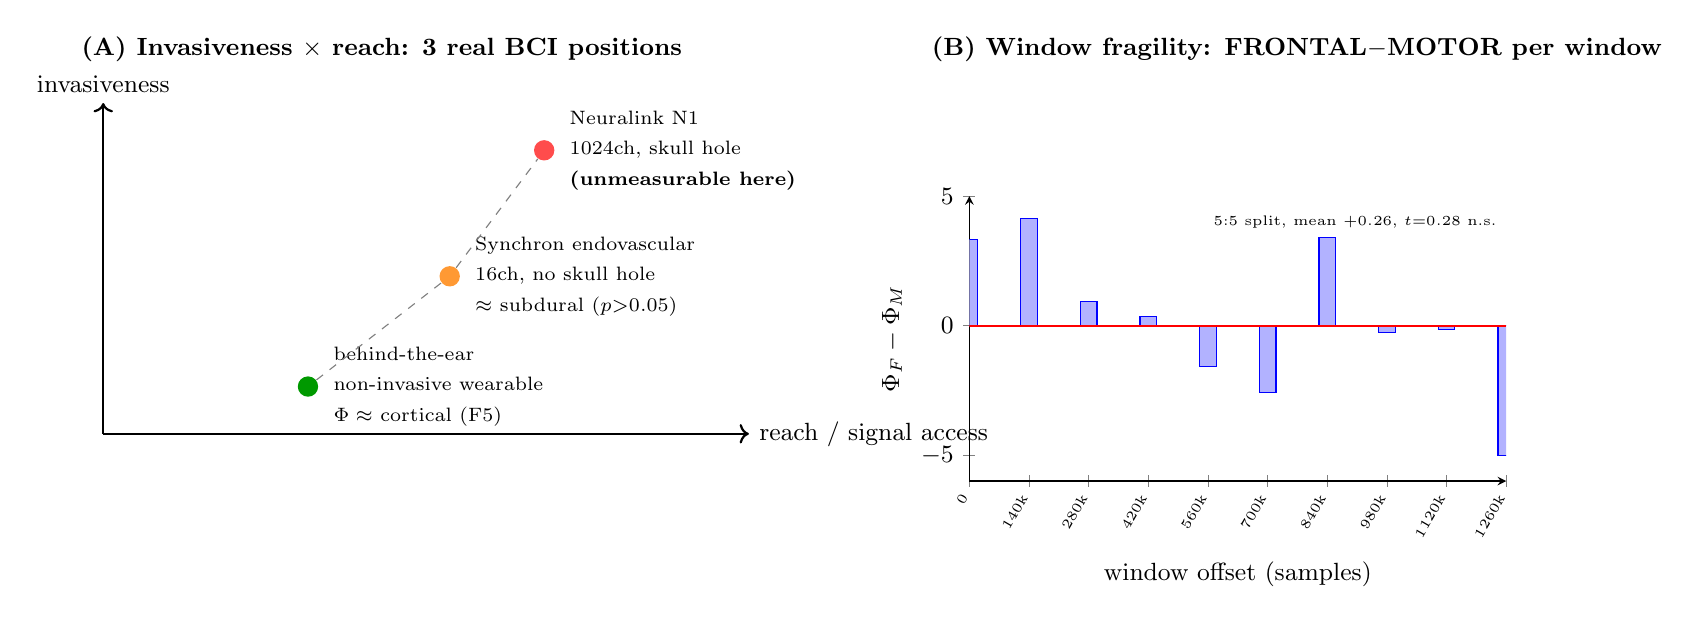
\begin{tikzpicture}[font=\small]

% ===== Panel A: invasiveness x reach 3-position ladder =====
\begin{scope}
  \node[anchor=south west] at (-0.4,4.6) {\textbf{(A) Invasiveness $\times$ reach: 3 real BCI positions}};
  \draw[->,thick] (0,0) -- (8.2,0) node[right] {reach / signal access};
  \draw[->,thick] (0,0) -- (0,4.2) node[above] {invasiveness};

  \node[circle,fill=red!70,inner sep=2.6pt] (n1) at (5.6,3.6) {};
  \node[circle,fill=orange!80,inner sep=2.6pt] (syn) at (4.4,2.0) {};
  \node[circle,fill=green!60!black,inner sep=2.6pt] (ear) at (2.6,0.6) {};

  \node[align=left,anchor=west] at (5.8,3.6) {\scriptsize Neuralink N1\\ \scriptsize 1024ch, skull hole\\ \scriptsize \textbf{(unmeasurable here)}};
  \node[align=left,anchor=west] at (4.6,2.0) {\scriptsize Synchron endovascular\\ \scriptsize 16ch, no skull hole\\ \scriptsize $\approx$ subdural ($p{>}0.05$)};
  \node[align=left,anchor=west] at (2.8,0.6) {\scriptsize behind-the-ear\\ \scriptsize non-invasive wearable\\ \scriptsize $\Phi\approx$ cortical (F5)};

  \draw[dashed,gray] (ear) -- (syn) -- (n1);
\end{scope}

% ===== Panel B: window-fragility 5:5 split =====
\begin{scope}[xshift=11cm]
  \node[anchor=south west] at (-0.6,4.6) {\textbf{(B) Window fragility: FRONTAL$-$MOTOR per window}};
  \begin{axis}[
      at={(0,-0.6cm)},
      width=8.4cm, height=5.2cm,
      ybar, bar width=6pt,
      ymin=-6, ymax=5,
      xtick=data,
      xticklabel style={rotate=60,anchor=east,font=\tiny},
      symbolic x coords={0,140k,280k,420k,560k,700k,840k,980k,1120k,1260k},
      ylabel={$\Phi_{F}-\Phi_{M}$},
      xlabel={window offset (samples)},
      axis lines=left,
      every axis plot/.append style={fill=blue!55},
    ]
    \addplot coordinates {
      (0,3.326) (140k,4.141) (280k,0.924) (420k,0.366) (560k,-1.579)
      (700k,-2.583) (840k,3.400) (980k,-0.275) (1120k,-0.147) (1260k,-5.020) };
    \draw[red,thick] (axis cs:0,0) -- (axis cs:1260k,0);
    \node[anchor=north east,font=\tiny] at (axis cs:1260k,4.6)
      {5:5 split,\ mean $+0.26$,\ $t{=}0.28$\ n.s.};
  \end{axis}
\end{scope}

\end{tikzpicture}
}
\caption{\textbf{(A)} The three real BCI positions on an invasiveness$\times$reach
ladder: N1 intracortical ($\mu$m, skull hole, the one position we cannot
measure here) $>$ Synchron endovascular (mm, ECoG-grade, no skull hole,
$\approx$ subdural at $p{>}0.05$) $>$ behind-the-ear non-invasive
(cm; $\Phi\approx$ cortical, F5). \textbf{(B)} Window fragility: FRONTAL$-$MOTOR
$n{=}4$ big-$\Phi$ per window over the full 300\,s; the sign flips repeatedly,
giving a $5{:}5$ split, mean $+0.26$, $t(9){=}0.28$ n.s.\ --- the
non-stationarity that dissolves the position effect (Table~\ref{tab:f1}).}
\label{fig:ladder}
\end{figure}

The practical bypass is not relocation \emph{among} cortical positions (null,
F1) but lowering \emph{invasiveness} along a real device ladder
(Fig.~\ref{fig:ladder}):
\begin{itemize}\itemsep0pt
  \item \textbf{N1 intracortical} --- penetrating, 1024 ch, skull hole; highest
  invasiveness, the only position with true $\mu$m/deep access (but the very
  thing we cannot measure).
  \item \textbf{Synchron endovascular} --- 16 ch in the superior sagittal
  sinus, no skull hole; PMC5976775 reports endovascular $\approx$ subdural
  $\approx$ epidural in bandwidth/SNR/decoding ($p{>}0.05$), i.e.\ \emph{ECoG-grade}
  signal from inside a vein; COMMAND trial $6/6$ primary endpoints.
  \item \textbf{Behind-the-ear (post-aural)} --- non-invasive wearable; its
  $n{=}4$ big-$\Phi$ is statistically equivalent to cortical positions (F5).
\end{itemize}
The ordering N1 $>$ Synchron($\approx$ECoG) $>$ behind-the-ear is an
invasiveness gradient, and our measurements say the \emph{reach} difference
across it is not visible at the scalp-proxy big-$\Phi$ level --- which is itself
the argument for the least-invasive option when the goal is integrated-info
read-out rather than deep stimulation.

\subsection{(e) Intracortical ceiling --- explicit scope boundary}
See Section~\ref{sec:ceiling}.

% =========================================================================
\section{The intracortical ceiling (scope boundary, not a to-do)}
\label{sec:ceiling}

The relocate thesis ultimately asks an \emph{intracortical} causal question:
``if the actual N1 electrode is moved from M1 to DLPFC, does whole-brain
control follow?'' No scalp or endovascular proxy can answer it. Three barriers
are physical/ethical, not engineering gaps:

\begin{table}[h]
\centering
\caption{Why the proxy can never close the intracortical question
(\texttt{AURA/B7-intracortical-ceiling.md}).}
\label{tab:ceiling}
\small
\begin{tabular}{@{}lp{7.2cm}l@{}}
\toprule
barrier & content & bypassable? \\
\midrule
spatial resolution & scalp $\sim$cm; endovascular $\sim$mm; intracortical
$\sim\mu$m (single-neuron) --- the integration resolution itself differs &
no (physics) \\
deep access & proxies see cortical surface / vein only; VTA/LC/raphe direct
signal is zero (even endovascular is a surface) & no (physics) \\
cause vs.\ correlation & proxy only observes; ``move position $\to$ stimulate
$\to$ effect'' needs invasive stimulation & no (ethics: human-invasive) \\
\bottomrule
\end{tabular}
\end{table}

\noindent
Therefore the remaining frontier --- animal invasive recording
(NHP optogenetic DLPFC$\to$VTA), or clinical N1/Utah/Stentrode patient raw ---
sits \emph{above} our lane, behind a physical and an IRB/regulatory wall. We
record this as the domain's \textbf{terminal boundary}, not as ``done'':
proxy + structure-model questions are closed; intracortical placement is
\emph{explicitly out of scope}. This is the honest scope line of a
negative-result paper.

% =========================================================================
\section{Verdict matrix}\label{sec:verdicts}

\begin{table}[h]
\centering
\caption{Every section claim, its tier, and its persisted verdict pointer
(\texttt{a\_paper\_sections}). Tiers: \tierGreen{} numerical, \tierRed{}
closed-negative.}
\label{tab:matrix}
\small
\begin{tabular}{@{}llll@{}}
\toprule
claim & tier & section & \texttt{.verdicts/} pointer \\
\midrule
F1 position null ($5{:}5$, $t{=}0.28$) & \tierRed & \ref{sub:f1} &
\texttt{a10-window-stats/test.txt} \\
F2 state null (awake vs sed) & \tierRed & \ref{sub:f2} &
\texttt{b2-postaural-state/awake\_vs\_sed.txt} \\
F4 multi-subject $\alpha$ $0/3$ & \tierRed & \ref{sub:f4} &
\texttt{b6-multisubject-alpha/run.txt} \\
B4.1 single-subject $\alpha$ trend & \tierRed & \ref{sub:f4} &
\texttt{b4-metric-sweep/alpha\_power\_state.txt} \\
F5 post-aural $\approx$ cortical & \tierGreen & \ref{sub:f5} &
\texttt{b1-postaural/viability.txt} \\
F3 reach$\to\Phi$ monotone & \tierGreen & \ref{sub:f3} &
\texttt{a7-reach-to-phi/curve.txt} \\
A6 relocate $\Delta\Phi{=}{+}17.66$ & \tierGreen & \ref{sub:f3} &
\texttt{a6-bigphi-closed-loop/relocate\_bigphi.txt} \\
A7 coupling robustness $6/6$ & \tierGreen & \ref{sub:f3} &
\texttt{a7-coupling-robustness/sweep.txt} \\
A8 literature connectome order & \tierGreen & \ref{sub:f3} &
\texttt{a8-connectome-coupling/run.txt} \\
A9 real Allen connectome order & \tierGreen & \ref{sub:f3} &
\texttt{a9-tractography/run.txt} \\
A8.1 single-window montage mirage & \tierGreen & \ref{sub:f3} &
\texttt{a8-montage-position/run.txt} \\
\bottomrule
\end{tabular}
\end{table}

% =========================================================================
\section{Related positions and limitations}\label{sec:limits}

\paragraph{Limitations (honest).}
(1) All real-EEG big-$\Phi$ is $n{=}4$ \emph{scalp-proxy} --- not intracortical,
low absolute magnitude. (2) F1/F2/F5 are single-subject (\texttt{sub-1010});
F4 is $N{=}3$, still small, though the $0/3$ and $1/3$ direction counts plus two
strongly-negative subjects make the negative firm-to-suggestive. (3) The awake
condition is eyes-open, a real $\alpha$-suppression confound. (4) $n{\ge}6$
exact big-$\Phi$ is compute-walled locally and not attempted; multi-window
averaging or band-power features (not single-window IIT-4.0 $\Phi$) would be
the proper next estimator within the scalp lane. (5) The connectome ``real''
prior is mouse (Allen); human tractography would refine it but is not expected
to overturn the hub$>$M1 ordering.

\paragraph{Why this is a finding, not a non-result.}
Per \texttt{a\_paper\_negative\_ok}: a closed-negative that deterministically
rules out an axis is publishable. Here we rule out the \emph{scalp-proxy
measurability} of the relocate thesis and expose a structure$\leftrightarrow$measurement
asymmetry, while fixing the intracortical question as an explicit physical/ethical
boundary. The negative is the contribution.

% =========================================================================
\section{Conclusion}\label{sec:conclusion}

Moving the electrode does not, on real human scalp EEG, change a single-window
$n{=}4$ big-$\Phi$ read of integrated information by either position or state,
and the one spectral trend that looked promising in one subject does not
replicate across three. The relocate thesis is nonetheless structurally
coherent: every in-silico and connectome model --- including the real Allen
connectome --- favours a projection hub over M1. That dissociation,
structure-favoured $\perp$ measurement-null, is the finding. The practical
corollary is an invasiveness ladder (N1 $>$ Synchron $\approx$ ECoG $>$
behind-the-ear) on which the reach difference is invisible at the scalp-proxy
big-$\Phi$ level, and a hard ceiling: the actual intracortical relocation
question is permanently outside a scalp/endovascular proxy's reach, for reasons
of physics and ethics rather than engineering.

% =========================================================================
\appendix
\section{Reproduction}\label{app:repro}
All verdicts are persisted raw \texttt{hexa verify}/run stdouts under
\texttt{.verdicts/} (pointers in Table~\ref{tab:matrix}); the structure-layer
toys are at \texttt{AURA/toy/*.hexa}; the multi-subject $\alpha$ harness is
\texttt{AURA/toy/b6\_multisubject\_alpha.py}; the dataset is OpenNeuro
\texttt{ds005620} (\texttt{aws s3 --no-sign-request}). Domain narrative and the
provenance pointer table are in \texttt{AURA/} (\texttt{SURVEY.md},
\texttt{A10-window-stats.md}, \texttt{B1}--\texttt{B7}).

\bibliographystyle{plainnat}
\bibliography{references}

\end{document}
